\documentclass[a4paper,11pt, twoside]{article}
\usepackage[english]{babel}
%\usepackage[utf8]{inputenc}
\usepackage{amsmath}
\usepackage{graphicx}
\usepackage{float}
\usepackage{fixltx2e}
\usepackage{listings}
\usepackage{enumitem}
\usepackage{color}
\usepackage{textcomp}
\usepackage{latexsym}
\usepackage{lstautogobble}
\usepackage[colorinlistoftodos]{todonotes}
\usepackage[margin=3cm]{geometry}
\usepackage{hyperref}
\usepackage{fancyhdr}
\usepackage{dirtree}
\usepackage{tikz}
\usetikzlibrary{patterns}
\usetikzlibrary{shapes,positioning,calc}
\usetikzlibrary{shapes.geometric, arrows}
\usetikzlibrary{arrows.meta}
\colorlet{lightgray}{gray!20}
\usepackage{libertine}
\usepackage{csquotes}
\usepackage[backend=bibtex, style=numeric]{biblatex}
\addbibresource{biblio.bib}
\hypersetup{
	hidelinks, 
	colorlinks = true,
	linkcolor = black,
	citecolor = black,
	urlcolor = blue
}
\lstset{
language=Java,
keywordstyle=\color{blue},
showtabs=false,
showspaces=false,
showstringspaces=false,
numbers=left,
frame=single,
basicstyle=\ttfamily\footnotesize,
breaklines=true,
tabsize=2,
escapeinside={(*@}{@*)}
}

\pagestyle{fancy}
\lhead{\nouppercase{\leftmark}}
\rhead{\nouppercase{\rightmark}}
\chead{}
\lfoot{}
\cfoot{\thepage}
\rfoot{}
\renewcommand{\headrulewidth}{0.4pt}
\renewcommand*\DTstylecomment{\rmfamily}

\renewcommand{\ttdefault}{cmtt}
\begin{document}
	\clearpage
	\begin{titlepage}
		\centering
		\vspace*{\fill}
		{\scshape\LARGE University of Verona \par}
		\vspace{1.5cm}
		\line(1,0){240} \\
		{\huge\bfseries Authorship Attribution\par}
		\line(1,0){240} \\
		\vspace{0.5cm}
		{\scshape\Large Big Data project report\par}
		\vspace{2cm}
		{\Large\itshape Davide Bianchi VR424505\par
		\Large\itshape Matteo Danzi VR424987\par}
		\vspace{1cm}
		\vspace{5cm}
		\vspace*{\fill}
		% Bottom of the page
		{\large A.Y. 2018/2019\par}
	\end{titlepage}
	\thispagestyle{empty}
	\newpage
	\tableofcontents
	\newpage
	
	\section{Introduction}
	The project aim was to design a tool which could establish the authorship of a manuscript by using specific criteria described later. 
	The used architecture is based on Hadoop, a distributed filesystem simulator, running in a Docker container. The requirements of the project imposed the use of MapReduce programming model as seen in Laboratory Lessons of the Big Data course.

	\section{Background and System Description}
    \subsection{Cloudera Docker and system setup}
		A container is a standard unit of software that packages up code and all its dependencies so the application runs quickly and reliably from one computing environment to another. A Docker container image is an executable package of software that includes everything needed to run an application: code, runtime, system tools, system libraries and settings.

		\bigskip

		\noindent
		Docker images become containers when they run on Docker Engine. They isolate software from its environment and ensure that it works uniformly despite differences for instance between development and staging.
		
		\bigskip

		\noindent
		The Cloudera\parencite{Cloudera} Docker image used in this project contains an Hadoop Distributed File System (HDFS) partition. Cloudera provides a scalable, flexible, integrated platform that makes it easy to manage rapidly increasing volumes and varieties of data in an enterprise. 

		\bigskip
		
		\noindent
		Cloudera provides an HDFS (\textit{Hadoop Distributed FileSystem})\parencite{Hadoop-Mapreduce}, used to store files across server collections. The Hadoop version used in this project is \texttt{Hadoop 2.6.0-cdh5.7.0}.
		
		The distributed filesystem consists on two basic services: \begin{itemize}
			\item \textit{NameNode}: is a single instance service, running on a master node, which is responsible for files and directory mantainance within the filesystem itself;
			
			\item \textit{DataNode}: running on multiple nodes (many instances are allowed), are supposed to retrieve the application data when they are told by the NameNode.
		\end{itemize}
		\begin{figure}[h!]
			\centering
			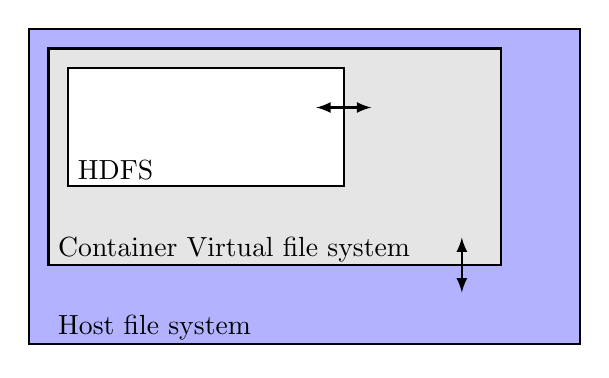
\begin{tikzpicture}[>=latex]
				\fill[draw=black, thick, fill=blue!30!white] (0,0) rectangle (7,4);\node[anchor=west] at (0.25,0.2) {Host file system};
				\fill[draw=black, thick, fill=lightgray] (0.25,1) rectangle (6,3.75);\node[anchor=west] at (0.25,1.2) {Container Virtual file system};
				\fill[draw=black, thick, fill=white] (.5,2) rectangle (4,3.5);\node[anchor=west] at (0.5,2.2) {HDFS};
				\draw[<->,thick] (5.5,.65) -- (5.5,1.35);\draw[<->,thick] (3.65,3) -- (4.35,3);
			\end{tikzpicture}
			\caption{File system organization}
			\label{tikz:filesys}
		\end{figure}

		For the installation of Docker, the Cloudera Docker image and the execution of jobs using jar file it have been used the instructions of the course. The project is written using Java version \texttt{11.0.4}. For the code compilation we used IntelliJ version \texttt{2019.2.4} compiling using compatibility mode with version \texttt{1.7}.

		

	\subsection{Map Reduce Framework}
		MapReduce is a programming paradigm which works on parallel platforms in order to process in the best possible way large amounts of data. The client has to implement a map function, which is supposed to take as input raw data and process them into intermediate \textit{key-value} pairs, and the reduce function, which aim is to regroup key-value pairs relying on the key and generate key-value output pairs. The mapreduce model is explained more in detail in the next section.
		
		\bigskip


		\noindent
		This Programming Model consists of two main actions:
		\begin{itemize}
			\item \textbf{Map}: application of a function to every object in a list. Each object (e.g.: document) is independent.
			\begin{itemize}
				\item Order is not important
				\item Maps can be done in parallel since every object has no relation to each other
				\item The function produces an intermediate result
			\end{itemize}
			
			Formally the \textit{map} function can be described with the following notation: \[ map:(key_1, value_1) \to list(key_2, value_2) \]
			\item \textbf{Reduce}: grouping key-value pairs on key, and combining the intermediate results generated by Maps to produce a final result. Formally the reduce function is defined as \[ reduce:(key_2, list(value_2)) \to (key_3, value_3)  \]
		\end{itemize}

		\begin{figure}[h!]
			\centering
			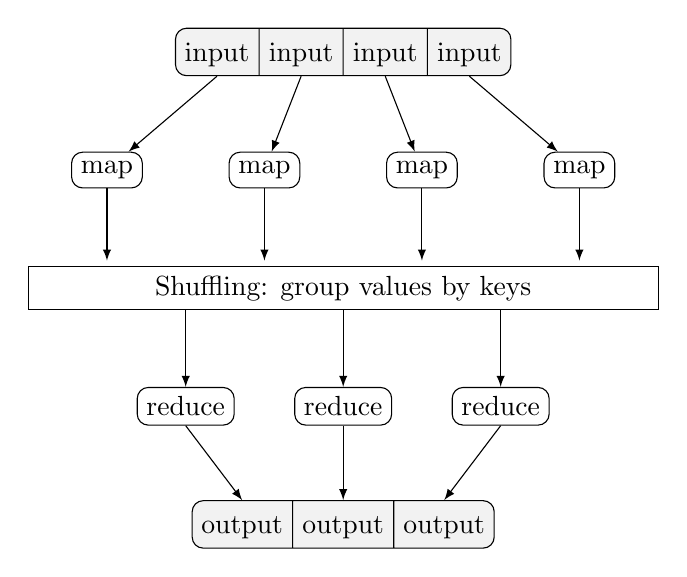
\begin{tikzpicture}[>=latex, relation/.style={rectangle split, rectangle split parts=#1, rectangle split part align=base, draw, anchor=center, align=center, text height=3mm, text centered}]
				% Nodes

				\node [relation=4, rounded corners, rectangle split horizontal, rectangle split part fill={lightgray!50}] (n0) at (0,0)
				{%
					\nodepart{one} input
					\nodepart{two} input
					\nodepart{three} input
					\nodepart{four} input};
				\node [draw, rectangle, rounded corners] (m1) at (-3,-1.5) {map};
				\node [draw, rectangle, rounded corners] (m2) at (-1,-1.5) {map};
				\node [draw, rectangle, rounded corners] (m3) at (1,-1.5) {map};
				\node [draw, rectangle, rounded corners] (m4) at (3,-1.5) {map};
				\draw node[draw, rectangle, minimum width=8cm] (inter) at ($ (n0) +(0,-3) $) {Shuffling: group values by keys};
				\node [draw, rectangle, rounded corners] (r1) at (-2,-4.5) {reduce};
				\node [draw, rectangle, rounded corners] (r2) at (0,-4.5) {reduce};
				\node [draw, rectangle, rounded corners] (r3) at (2,-4.5) {reduce};
				\node [relation=3, rounded corners, rectangle split horizontal, rectangle split part fill={lightgray!50}] (n1) at (0,-6)
				{%
					\nodepart{one} output
					\nodepart{two} output
					\nodepart{three} output};

				% Arrows

				\draw[->] (n0.one south) -- (m1);\draw[->] (n0.two south) -- (m2);
				\draw[->] (n0.three south) -- (m3);\draw[->] (n0.four south) -- (m4);
				\draw[->] (m1) -- +(0,-1.15);\draw[->] (m2) -- +(0,-1.15);
				\draw[->] (m3) -- +(0,-1.15);\draw[->] (m4) -- +(0,-1.15);
				\draw[->] ($ (inter.south) +(-2,0) $) -- (r1);\draw[->] (inter.south) -- (r2);
				\draw[->] ($ (inter.south) +(2,0) $) -- (r3);
				\draw[->] (r1.south) -- (n1.one north);
				\draw[->] (r2.south) -- (n1.two north);
				\draw[->] (r3.south) -- (n1.three north);
			\end{tikzpicture}
			\caption{MapReduce Model}
    		\label{tikz:mapred}
		\end{figure}
	
	\newpage
	\section{Project workflow and structure}
	The first step of the project is to analyze an amount of manuscripts, extracting relevant information from them in order to create a ``dictionary'' of known authors. It performs the calculation of the frequencies of language parts used by the authors in their texts. Starting from these data, the following steps consist of taking unknown manuscripts as input and establishing the authorship by the comparing them with the ``dictionary'' previously created. 
	
	All the manuscripts are \texttt{.txt} files taken from the Project Gutenberg\parencite{Gutenberg} online library.
	The Project Workflow is the following:
	\begin{enumerate}
		\item Parsing all the files using Hadoop Map Reduce job: 
		\begin{enumerate}
			\item Mapper performs the counting of all the specified language parts in each file. These parts are ArrayList instances. The Mapper associates each language part with an integer flag set to 1. The collected data are explained more in detail in the next sections. 
			
			\item Reducer performs the counting of language parts by putting together data taken from the Mappers. The reducer output  
		\end{enumerate}
		\item Calculating the frequencies of language parts for each text.
		\item Obtaining an author ``identikit'' based on the texts that have been analyzed written by that specific author. The author characteristics are built merging the data resulting from the text analysis.
		\item Analyzing unknown texts and comparing them to the known author is order to have a rank of similarity between the unknown texts and the known authors.
	\end{enumerate}

	\subsection{Project structure}
	The project main folder is divided in the following directories:
	\begin{figure}[h!]
		\dirtree{%
			.1 big-data-project. 
			.2 doc\DTcomment{generated javadoc folder}. 
			.2 libs \DTcomment{Hadoop libraries}. 
			.2 report\DTcomment{project report}. 
			.2 src \DTcomment{code sources}. 
			.3 main. 
			.4 java. 
			.5 AffinityMap.java. 
			.5 Authorship.java. 
			.5 FreqMap.java. 
			.5 FreqMapEntry.java. 
			.5 Main.java. 
			.5 SimilarityAnalysis.java. 
		}
	\end{figure}

	\subsection{Map Reduce Job}
	The project only contains a single mapreduce job, alongside with other classes to hold temporary data. The mapreduce job is implemented in a single class named \lstinline|Authorship|. In order to proceed with the implementation, the code has to import several libraries, which provide interface to the HDFS functions. These libraries are:
	\begin{figure}[h!]
		\dirtree{%
			.1 libs. 
			.2 hadoop-annotations.jar. 
			.2 hadoop-common.jar. 
			.2 hadoop-core-2.6.0-mr1-cdh5.7.0.jar. 
			.2 hadoop-hdfs.jar. 
			.2 log4j-1.2.17.jar. 
		}
	\end{figure}

	Before diving into the implementation of the job, we have to assure that the current class (compiled into a \verb|jar| file), will run as an hadoop job. In order to do so, we have to add \lstinline|extends Configured implements Tool| to the class declaration.
	
	\bigskip
	\noindent
	As said in the previous sections, the client has to manually implement the map and the reduce functions, alongside with a \lstinline|run| method to configure the job itself.

	\subsubsection{Run method}
	Contains the job configuration, setting input and output paths.
	The job is configured as follows:
	
	\begin{lstlisting}[firstnumber=45, caption={Run method}, captionpos=b]
@Override
public int run(String[] args) throws Exception {
	Job job = Job.getInstance(this.getConf(), "authorship");
	job.setJarByClass(this.getClass());
	TextInputFormat.setInputPaths(job, new Path(INPUT_PATH));
	TextInputFormat.setInputPaths(job, new Path(UNKNOWNS_INPUT_PATH));
	TextOutputFormat.setOutputPath(job, new Path(OUTPUT_PATH));
	
	for (String s : Main.buildPaths(this))
		FileInputFormat.addInputPath(job, new Path(s));
	
	job.setMapperClass(Map.class);
	job.setCombinerClass(Reduce.class);
	job.setReducerClass(Reduce.class);
	job.setMapOutputKeyClass(Text.class);
	job.setMapOutputValueClass(IntWritable.class);
	job.setOutputKeyClass(Text.class);
	job.setOutputValueClass(IntWritable.class);
	
	return job.waitForCompletion(true) ? 0 : 1;
}
	\end{lstlisting}
	
	Note that several costants are used: \begin{itemize}
		\item \lstinline|INPUT_PATH| is the input path for known texts;
		\item \lstinline|OUTPUT_PATH| is the reduce output path;
		\item \lstinline|UNKNOWNS_INPUT_PATH| is the input path for unknown texts (which are located in a subdirectory of \lstinline|INPUT_PATH|).
	\end{itemize}

	The calls to \lstinline|setInputPaths| and \lstinline|setOutputPath|, as the name suggests, are used to set respectively the input and output paths of the job. We then add the single files using a call to \lstinline|addInputPath| for each input file we have. 
	
	\bigskip
	\noindent
	In the following lines, we configure the mapper and reducer input and output types and classes.
	Respectively: \begin{itemize}
		\item mapper output key is \lstinline|Text| (the hadoop-like type for \lstinline|String|);
		\item mapper output value is \lstinline|IntWritable| (standing for \lstinline|Integer|);
		\item reducer output key is \lstinline|Text|;
		\item reducer output value is \lstinline|Integer|.
	\end{itemize}

	Calls to \lstinline|job.setMapperClass|, \lstinline|job.setReducerClass| and \lstinline|job.setCombinerClass| just tell the interpreter which is the class respinsible for describing the mapping, reducing and combining function.
	
	\subsubsection{Mapper implementation.} The mapper is implemented in an inner class, and we can summarize the content by dividing it in three sections.
	
	The first one contains the declaration of patterns during the analysis.
	
	\begin{lstlisting}[firstnumber=70, caption={Declaration of Regular Expression Patterns}, captionpos=b]
private static final Pattern WORD_BOUNDARY = Pattern.compile("\\s*\\b\\s *");
private static final Pattern END_PERIOD = Pattern.compile("[a-z][.!?]");
private static final Pattern MARKS_COMMAS = Pattern.compile("[,!?]");
private static final Pattern DIALOGUE = Pattern.compile("[\u201C\u201D]");
private static final IntWritable ONE = new IntWritable(1);
	\end{lstlisting}
	
	These pattern are used in the text analysis. Briefly: \begin{itemize}
		\item \lstinline|WORD_BOUNDARY|: splits on word separators characters;
		\item \lstinline|END_PERIOD|: splits text on end-period characters;
		\item \lstinline|MARKS_COMMAS|: splits on commas and exclamation/question marks;
		\item \lstinline|DIALOGUE|: splits on dialogue quotes (\lstinline|\u201C| and \lstinline|\u201D| is their specification in Unicode, since these symbols are not in the standard ASCII table). 
	\end{itemize}

	The last constant is an \lstinline|IntWritable| value set to 1, and is used when a matching expression is detected.

	The second section contains the text analysis itself, which is based on: \begin{itemize}
		\item article, preposition and conjunction frequency;
		\item average period length;
		\item dialogues frequency;
		\item punctuation mark frequency.
	\end{itemize}
	Besides this, we save additional informations, such as the total number of words in the input and the total number of periods, so we can get the frequency over the total dimension of the input.

	In this section the previous pattern matchers are used to reach these words and write the corresponding \lstinline|ONE| in the job contest. 
	
	We report an example for articles count: \begin{lstlisting}[firstnumber=82, caption={Articles counting in Map method}, captionpos=b]
for (String word : WORD_BOUNDARY.split(lineText.toString())) {
	String refWord = word.toLowerCase();
	if (!word.isEmpty()) {
		if (Authorship.ARTICLES.contains(refWord) || refWord.startsWith("l'") || refWord.startsWith("un'") || refWord.startsWith("gl'")) {
		
			text.set(filePathString + "*article");
			context.write(text, ONE);
		}
	}

	...

}
	\end{lstlisting}
	
	In short terms, for each article found in the input text, the mapper writes a string formatted as follows:\begin{center}
		\textit{author-title.txt*article\textless tab\textgreater \textless value\textgreater} 
	\end{center}

	This procedure applies in the same way to preposition and conjunctions.
	
	\bigskip
	\noindent
	For periods, punctuation and dialogues we used a different method.
	\begin{lstlisting}[firstnumber=109, caption={Periods counting in Map method}, captionpos=b]
Matcher matcher = END_PERIOD.matcher(refLineText);
while (matcher.find()) {
	text.set(filePathString + "*periods");
	context.write(text, ONE);
}
	...
	\end{lstlisting}
	
	A \lstinline|Matcher| instance tries to match the pattern to an input line. As soon as the matcher finds occurences of the pattern in the text passed as parameter, the mapper writes a line similar to the previous one (i.e. formatted in the same way) to the context. The procedure repeats for punctuation marks, commas and periods delimitators.
	
	\subsubsection{Reducer implementation}
	The reducer implementation is pretty much the same as in the \lstinline|Wordcount| example. Since it's just a few lines we report the full code:
	\begin{lstlisting}[firstnumber=135, caption={Reduce method}, captionpos=b]
@Override
protected void reduce(Text key, Iterable<IntWritable> values, Context context) throws IOException, InterruptedException {
	int sum = 0;
	for (IntWritable count : values) {
		sum += count.get();
	}
	context.write(key, new IntWritable(sum));
}
	\end{lstlisting}
	
	Since the context has now a lot of lines associated with same value (the \lstinline|IntWritable| instance for ``ones''), the combiner and the reducer are responsible for grouping lines with the same key and count these lines, writing the total into the context.
	
	
	\subsection{Frequency Calculations}
	Once the hadoop job has terminated, the control passes to a simple Java program. This section of the program generates an instance of the class \lstinline|FreqMap| parsing the reducer output file.
	
	A \lstinline|FreqMap| instance is a set of \lstinline|FreqMapEntry|, which are entries text-specific. More in detail an instance of \lstinline|FreqMapEntry| consists of: \begin{itemize}
		\item a \lstinline|String| author name;
		\item a \lstinline|String| text title;
		\item a map \lstinline|String| $\to$ \lstinline|Float|, containing field names (text features extracted from the mapreduce framework) and their respective values.
	\end{itemize}

	More in detail, a complete entry contains the following fields: \begin{itemize}
		\item frequency of articles;
		\item frequency of prepositions;
		\item frequency of conjunctions;
		\item number of words in the input;
		\item number of periods in the input;
		\item frequency of punctuation marks;
		\item frequency of dialogue sentences.
		\item average period length.
	\end{itemize}

	Note that the frequency of articles, prepositions, cojunctions and punctuation symbols is determined over the total number of words, while the frequency of dialogue sentences is calculated over the total number of periods.
	
	After this phase, we will have a frequency map for every text of every author, for example: \begin{align*}
		\text{author}&: M. Shelley \\
		\text{title} &: Frankenstein \\
		\text{frequencies}&:\begin{cases}
			articles &0.07756892 \\
			prepositions &0.11023554 \\
			conjunctions &0.037609607 \\
			periods &3441 \\
			nwords &69796.0 \\
			avg\text{-}period\text{-}length &20.283638 \\
			commas &0.079789676 \\
			dialogues &0.112322
		\end{cases}
	\end{align*}
	 What we need now is a map of frequencies relative to a single author, order to generate a ``stylistic identikit''  of an author, so then we can compare any unknown text to that author.
	 
	 In order to do so we pick all the informations we got about every known text of every author and we merge this maps into a single one, which is relative to an author. That is, if we have multiple texts of the same author, we generate a new \lstinline|FreqMapEntry|, were the author remains the same, but we set as title a \lstinline|String| set to the value \lstinline|"global"|, in order to identify that map as the author identikit we were talking some lines above.
	 
	 \bigskip
	 \noindent
	 The global entries are generated with the following method.
	 \begin{lstlisting}[firstnumber=79, caption={globalAuthorFrequency method}, captionpos=b]
private void globalAuthorFrequency(String author) {
	FreqMapEntry global = new FreqMapEntry(author, "global");(*@\label{eighty}@*)
	
	// init map to 0
	for (String field : entries.iterator().next().getFrequencies().keySet()) {
		global.getFrequencies().put(field, (float) 0);(*@\label{eightyfour}@*)
	}
	
	// sums by field, entries are grouped by author
	int authorEntries = 0;(*@\label{eightyeight}@*)
	for (FreqMapEntry entry : this.entries) {
		if (entry.getAuthor().equals(author)) {
			authorEntries++;
			for (String field : entry.getFrequencies().keySet()) {
				float upvalue = global.getFrequencies().get(field) + entry.getFrequencies().get(field);
				global.getFrequencies().put(field, upvalue);(*@\label{ninetyfour}@*)
			}
		}
	}
	
	// average using number of entries
	for (String field : global.getFrequencies().keySet()) {(*@\label{100}@*)
		global.getFrequencies().put(field, global.getFrequencies().get(field) / authorEntries);
	}(*@\label{102}@*)
	
	this.entries.add(global);
}
	 \end{lstlisting}
	 
	 The methods proceeds following these steps: \begin{enumerate}
	 	\item lines \ref{eighty} :: \ref{eightyfour} build the map reserved for the complexive values of the author, and initializes all the fields to 0;
	 	\item lines \ref{eightyeight} :: \ref{ninetyfour} query all the previous instances of \lstinline|FreqMap| entry, get a specific field value and sum this value to all other matching fields in other instances.
	 	\item lines \ref{100} :: \ref{102} generate an average value for the global entry, dividing the sums obtained at the previous step by the total number of entries with the specific author name.
	 \end{enumerate}
	 
	 \bigskip
	 \noindent
	 At the end we will have in the beginning \lstinline|FreqMap| instance an entry for each text of each author and a global entry for every author.
	
	\subsection{Similarity Analysis}
	The last phase of the working project is the design of the mechanism which allows to attribute an hypotethic author to an unknown text.
	
	The task is done through the following steps: \begin{enumerate}
		\item generating a partial comparison between every couple of unknown text-known author;
		\item sorting this comparisons in order to get the most similar couples as the most correlated author to each unknown text.
	\end{enumerate}

	This steps are implemented in \lstinline|AffinityMap| and \lstinline|SimilarityAnalysis| classes.
	
	 An \lstinline|AffinityMap| instance represents a comparison of authors, the first is known and the second is not. The compared fields are represented as a map \lstinline|String| $\to$ \lstinline|Double|, as in previous classes. The \lstinline|AffinityMap| instance implements the \lstinline|Comparable| interface, in order to be able to compare two instances and determine a sort of ``hierarchy''.
	 
	 The comparison method is the following:\begin{lstlisting}[firstnumber=51,caption={AffinityMap comparison method}, captionpos=b, label={lst:comparemethod}]
@Override
public int compareTo(Object o) {
	AffinityMap rec = (AffinityMap) o;
	HashMap<Integer, Integer> count = new HashMap<>();(*@\label{54}@*)
	count.put(-1, 0);
	count.put(0, 0);
	count.put(1, 0);(*@\label{57}@*)
	
	// count for compare values
	for (String s : this.map.keySet()) {(*@\label{60}@*)
		if (this.map.get(s) < rec.map.get(s)) {
			count.put(-1, count.get(-1) + 1);
		} else if (rec.map.get(s) < this.map.get(s)) {
			count.put(1, count.get(1) + 1);
		} else {
			count.put(0, count.get(0) + 1);
		}
	}(*@\label{68}@*)
	
	// max on compare counts
	Map.Entry<Integer, Integer> max = null;
	int intmax = 0;(*@\label{72}@*)
	for (Map.Entry<Integer, Integer> entry : count.entrySet()) {
		if (entry.getValue() > intmax) {
			intmax = entry.getValue();
			max = entry;
		}
	}(*@\label{78}@*)
	assert max != null;
	return max.getKey();

}
	 \end{lstlisting}
	 
	 The code here is not clearly readable, we break it down to its basics. Before we dive into it, we have to recall the functioning of the standard \lstinline|compareTo(Object o)| method, inherited from the \lstinline|Comparable| interface. This method returns \begin{itemize}
	 	\item $0$ if the objects are equal;
	 	\item $-1$ if \lstinline|this| object is lower then the parameter object;
	 	\item $1$ if \lstinline|this| object is greater then the parameter object;
	 \end{itemize}
 
 	Now we can explain the code more in detail: \begin{itemize}
 		\item lines \ref{54} :: \ref{57} initialize to 0 three counters, one for each return type of the \lstinline|compare| method;
 		\item lines \ref{60} :: \ref{68} compare each field of the two maps (which have the same key) and increment the corresponding counter;
 		\item lines \ref{72} :: \ref{78} check which of the three counter has the maximum value; if $-1$ is the maximum, the current object is lower that the parameter item, if $1$ is the maximum the parameter item is lower than the current object, otherwise the two items are considered to be equal.
 	\end{itemize}
 
 	The comparison is ran from the method \lstinline|SimilarityAnalysis.exec()|, which is responsible for generating the correlations between unknown text and known authors and reporting to file the final rank. We start the description of the class from specifying how affinities are calculated, and report the \lstinline|exec()| method code.
 	
 	\begin{lstlisting}[firstnumber=38]
private void exec() {
	// remove non globals values and sort entries
	ArrayList<FreqMapEntry> unknowns = new ArrayList<>();
	ArrayList<FreqMapEntry> knowns = new ArrayList<>();
	
	for (FreqMapEntry entry : this.freqMap.getEntries()) {(*@\label{43}@*)
		if (entry.isUnknown() && entry.isGlobal()) {
			unknowns.add(entry);
		} else if (!entry.isUnknown() && entry.isGlobal()) {
			knowns.add(entry);
		}
	}
	
	// calc deltas for each FreqMapEntry combination
	for (FreqMapEntry kn : knowns) {
		for (FreqMapEntry unk : unknowns) {
			this.deltas.add(computedDelta(kn, unk));
		}
	}(*@\label{56}@*)
	
	Collections.sort(this.deltas, new Comparator<AffinityMap>() {(*@\label{58b}@*)
		// comparison method between two affinity maps, used to sort the analysis
		@Override
		public int compare(AffinityMap affinityMap, AffinityMap t1) {
			return affinityMap.compareTo(t1);
		}
	});(*@\label{64b}@*)
}
 	\end{lstlisting}
 	
 	\bigskip
 	\noindent
	As specified just few lines above, an \lstinline|AffinityMap| instance contains a map from String to doubles. Data in this map are saved as the field-to-field difference of the maps of the authors we are analyzing. More in detail, if we have two authors $A$ and $B$ (i.e. two \lstinline|FreqMapEntry| instances), the map will contain the following values (lines \ref{43} to \ref{56}):
	\begin{align*}
		\begin{cases}
			\text{articles} &= |A.\text{articles} - B.\text{articles}| \\
			\text{conjunctions} &= |A. \text{conjunctions}- B.\text{conjunctions}| \\
			\dots& \\
			\text{avg-period-length}&= |A.\text{avg-period-length} - B.\text{avg-period-length}|
		\end{cases}
	\end{align*}
	
	Lines \ref{58b} to \ref{64b} sort the collection of \lstinline|AffinityMap| instances using the \lstinline|compare| method described in listing \ref{lst:comparemethod}.
	
	The ranking is written to a new file in the HDFS (in directory \lstinline|OUTPUT_PATH|); the first position are the most similar, the last position are the smallest affinity pairs.
	
	
	
	

	
	
	\newpage
	\section{Performed tests}

	\newpage

	\printbibheading
	\printbibliography[nottype=book,heading=subbibliography,title={Online Sources}]





\end{document}